%%%%%%%%%%%%%%%%%%%%%%%%%%%%%%%%%%%%%%%%%
% Tufte-Style Book (Minimal Template)
% LaTeX Template
% Version 1.0 (5/1/13)
%
% This template has been downloaded from:
% http://www.LaTeXTemplates.com
%
% License:
% CC BY-NC-SA 3.0 (http://creativecommons.org/licenses/by-nc-sa/3.0/)
%
% IMPORTANT NOTE:
% In addition to running BibTeX to compile the reference list from the .bib
% file, you will need to run MakeIndex to compile the index at the end of the
% document.
%
%%%%%%%%%%%%%%%%%%%%%%%%%%%%%%%%%%%%%%%%%

%----------------------------------------------------------------------------------------
%	PACKAGES AND OTHER DOCUMENT CONFIGURATIONS
%----------------------------------------------------------------------------------------

\documentclass{tufte-book} % Use the tufte-book class which in turn uses the tufte-common class

\hypersetup{colorlinks} % Comment this line if you don't wish to have colored links

\usepackage{microtype} % Improves character and word spacing

\usepackage{lipsum} % Inserts dummy text

\usepackage{booktabs} % Better horizontal rules in tables

\usepackage{graphicx} % Needed to insert images into the document
\graphicspath{{graphics/}} % Sets the default location of pictures
\setkeys{Gin}{width=\linewidth,totalheight=\textheight,keepaspectratio} % Improves figure scaling

\usepackage{fancyvrb} % Allows customization of verbatim environments
\fvset{fontsize=\normalsize} % The font size of all verbatim text can be changed here

\newcommand{\hangp}[1]{\makebox[0pt][r]{(}#1\makebox[0pt][l]{)}} % New command to create parentheses around text in tables which take up no horizontal space - this improves column spacing
\newcommand{\hangstar}{\makebox[0pt][l]{*}} % New command to create asterisks in tables which take up no horizontal space - this improves column spacing

\usepackage{xspace} % Used for printing a trailing space better than using a tilde (~) using the \xspace command

\newcommand{\monthyear}{\ifcase\month\or January\or February\or March\or April\or May\or June\or July\or August\or September\or October\or November\or December\fi\space\number\year} % A command to print the current month and year

\newcommand{\openepigraph}[2]{ % This block sets up a command for printing an epigraph with 2 arguments - the quote and the author
\begin{fullwidth}
\sffamily\large
\begin{doublespace}
\noindent\allcaps{#1}\\ % The quote
\noindent\allcaps{#2} % The author
\end{doublespace}
\end{fullwidth}
}

\newcommand{\blankpage}{\newpage\hbox{}\thispagestyle{empty}\newpage} % Command to insert a blank page

\usepackage{makeidx} % Used to generate the index
\makeindex % Generate the index which is printed at the end of the document

%----------------------------------------------------------------------------------------
%	BOOK META-INFORMATION
%----------------------------------------------------------------------------------------

\title{A Proposal for an \\ Open Wireless \\ Sensor Network \\On-Line Course} % Title of the book

\author{Luis Sanabria et al.} % Author

\publisher{Universitat Pompeu Fabra} % Publisher

%----------------------------------------------------------------------------------------

\begin{document}

\frontmatter

%----------------------------------------------------------------------------------------
%	EPIGRAPH
%----------------------------------------------------------------------------------------

%\thispagestyle{empty}
%\openepigraph{Quotation 1}{Author, {\itshape Source}}
%\vfill
%\openepigraph{Quotation 2}{Author}
%\vfill
%\openepigraph{Quotation 3}{Author}

%----------------------------------------------------------------------------------------

\maketitle % Print the title page

%----------------------------------------------------------------------------------------
%	COPYRIGHT PAGE
%----------------------------------------------------------------------------------------

%\newpage
%\begin{fullwidth}
%~\vfill
%\thispagestyle{empty}
%\setlength{\parindent}{0pt}
%\setlength{\parskip}{\baselineskip}
%Copyright \copyright\ \the\year\ \thanklessauthor
%
%\par\smallcaps{Published by \thanklesspublisher}
%
%\par\smallcaps{\url{http://www.bookwebsite.com}}
%
%\par License information.\index{license}
%
%\par\textit{First printing, \monthyear}
%\end{fullwidth}

%----------------------------------------------------------------------------------------

\tableofcontents % Print the table of contents

%----------------------------------------------------------------------------------------

\listoffigures % Print a list of figures

%----------------------------------------------------------------------------------------

\listoftables % Print a list of tables

%----------------------------------------------------------------------------------------
%	DEDICATION PAGE
%----------------------------------------------------------------------------------------

%\cleardoublepage
%~\vfill
%\begin{doublespace}
%\noindent\fontsize{18}{22}\selectfont\itshape
%\nohyphenation
%Dedicated to my family and friends.
%\end{doublespace}
%\vfill
%\vfill

%----------------------------------------------------------------------------------------
%	INTRODUCTION
%----------------------------------------------------------------------------------------

\cleardoublepage
\chapter{Introduction} % The asterisk leaves out this chapter from the table of contents

It is a commonplace that the Internet is changing our lives.
It is changing the way we learn and also the way we contribute to our communities and organize ourselves.
In this course we will explore the bottom-up creation of a wireless sensor network that can be used to gather and share data.
This gathering and sharing of data empowers the citizenship to monitor and interact with the environment.

\begin{marginfigure}
\includegraphics[width=\linewidth]{SCK}
\caption{Smart Citizen Kit units. These are wireless nodes with multiple sensors.}
\label{fig:SCK}
\end{marginfigure}

We are interested in the bottom-up models.
We use the terms peer-to-peer, do-it-ourselves and bottom-up interchangeably.
The idea that we want to transmit with bottom-up is that the participant takes an active role and contributes to the community rather than being a mere consumer.
For this reason, we teach the first simple steps to build, configure and program a sensor that uploads the gathered data to the Internet to make it publicly available to those that are interested in.


%------------------------------------------------

\chapter{Methodology}

The course is organized in different units.
Each of the units is a basic ingredient in the construction of a bottom-up wireless sensor networks.
For each of the units, we will follow the same class dynamics.

\section{Class dynamics}

The course is divided into video lectures and written material, both published as the course goes on. Video content include: teaching lessons, interviews and additional instructions for the assignments (when necessary). While the written material is composed by assignments and quizzes. Further details are provided below.

Each unit starts with introductory video lessons in which the lecturer presents the different concepts, tools and examples that are going to be useful for both the assignments and quizzes.
Starting from the necessary theory underlying each unit, the lecturer then guides the students through hands-on examples providing further insight on the subject.

After each unit's video lessons, assignments and quizzes are "unlocked" to the student. Assignments are composed of written (and photographic) material detailing instructions on how to build examples, which work as hints to complete the assignment itself.

After completing the assignments, students are provided with all that is required to successfully complete the end-of-unit quizzes. These in turn are composed of both theory and assignment-related multiple-choice questions.

Teachers will propose challenges on each assignment, often composed of alternative or advanced services that can be added at various stages with little (or none) additional work. Challenges are not graded, but set the ground for a final course project which students may submit in order to gain additional credentials and compensate for previous assignments.

Challenges may be completed by forming groups of students, in fact, collaboration among groups is encouraged. It is strongly believed that discussion and feedback provide more valuable results and are considered as ways of effective learning in this platform.

%The participants will watch a motivation video and a video tutorial.
%The tutorial will describe how to complete a simple project and will be complemented.
%Then, the participants have to collaborate to solve a challenge.
%The teachers offer a suggested challenge, but the participants are free to take other challenges that are relevant to them and to the course.
%Finally, the participants have to carefully document their works so that it can be evaluated, reproduced and discussed by the other participants.

%The first and the last unit are slightly different.
%In the first unit there is no project as the focus is on the presentation of the participants, the course itself and the discussion of the expectations on the course.
%The last unit is also special because the participants design, plan, execute and document their own project. 
%The courses finishes with an exhibition of the personal projects.

\section{In-class courses}
Besides the online offering, the course will also offered in-class for students registered at Universitat Pompeu Fabra.
Furthermore it will be possible to use the material for Summer Schools to promote the University and Bottom-up Initiatives.

\section{Resources}


The course will be offered in the P2P University course platform.
The students will be offered with videos, a lab assignment guide with all the details of the different projects, and the discussion and feedback tools of the P2P University platform.
The guide will be adapted from the current guide for the existing in-class course on wireless sensor networks.

\begin{marginfigure}
\includegraphics[width=\linewidth]{p2pu}
\caption{The motto of the P2P University is ``Learn Anything with Your Peers''}
\label{fig:p2pu}
\end{marginfigure}

\section{Additional Material}

\begin{itemize}
\item Robert Faludi ``Building Wireless Sensor Networks''
\item Alejandro Andreu ``Open Sensor Network''
\end{itemize}


%------------------------------------------------

\chapter{Working Plan}

\begin{enumerate}
	\item Scripting of the course: preparation of the course structure including units segmentation, number/length of videos per unit, assignments and quiz dynamics and evaluation, feedback and collaboration management; and final project evaluation.
	\item Preparation of the written guide: there is already a guide for the in-class course, therefore this new adapted guide should take advantage of on-line resources (video, comments, etc.).
	\item Setting up the P2P University on-line platform: based on the course script, this task will configure the platform accordingly.
	\item Shooting and producing the videos: this final task aims at shooting the videos according to what was designed in the course script and configured in the P2P University platform.
\end{enumerate}


% \begin{itemize}
% \item Scripting of the course: Preparation of detailed scripts of the content of the videos, the guide and the requirements for the online platform.
% \item Shooting and producing the videos: The videos will be shot and produced according to the script.
% \item Preparation of the written guide: There is already a guide for the in-class course, but it needs to be adapted to the on-line course.
% \item Setting up the P2P University on-line platform: This task involves the actual creation and configuration of the online course.
% \end{itemize}

\begin{marginfigure}
\includegraphics[width=\linewidth]{video}
\caption{It is necessary to shoot videos with step-by-step instructions to build the pilots or complete the assignments.}
\label{fig:video}
\end{marginfigure}
\begin{marginfigure}
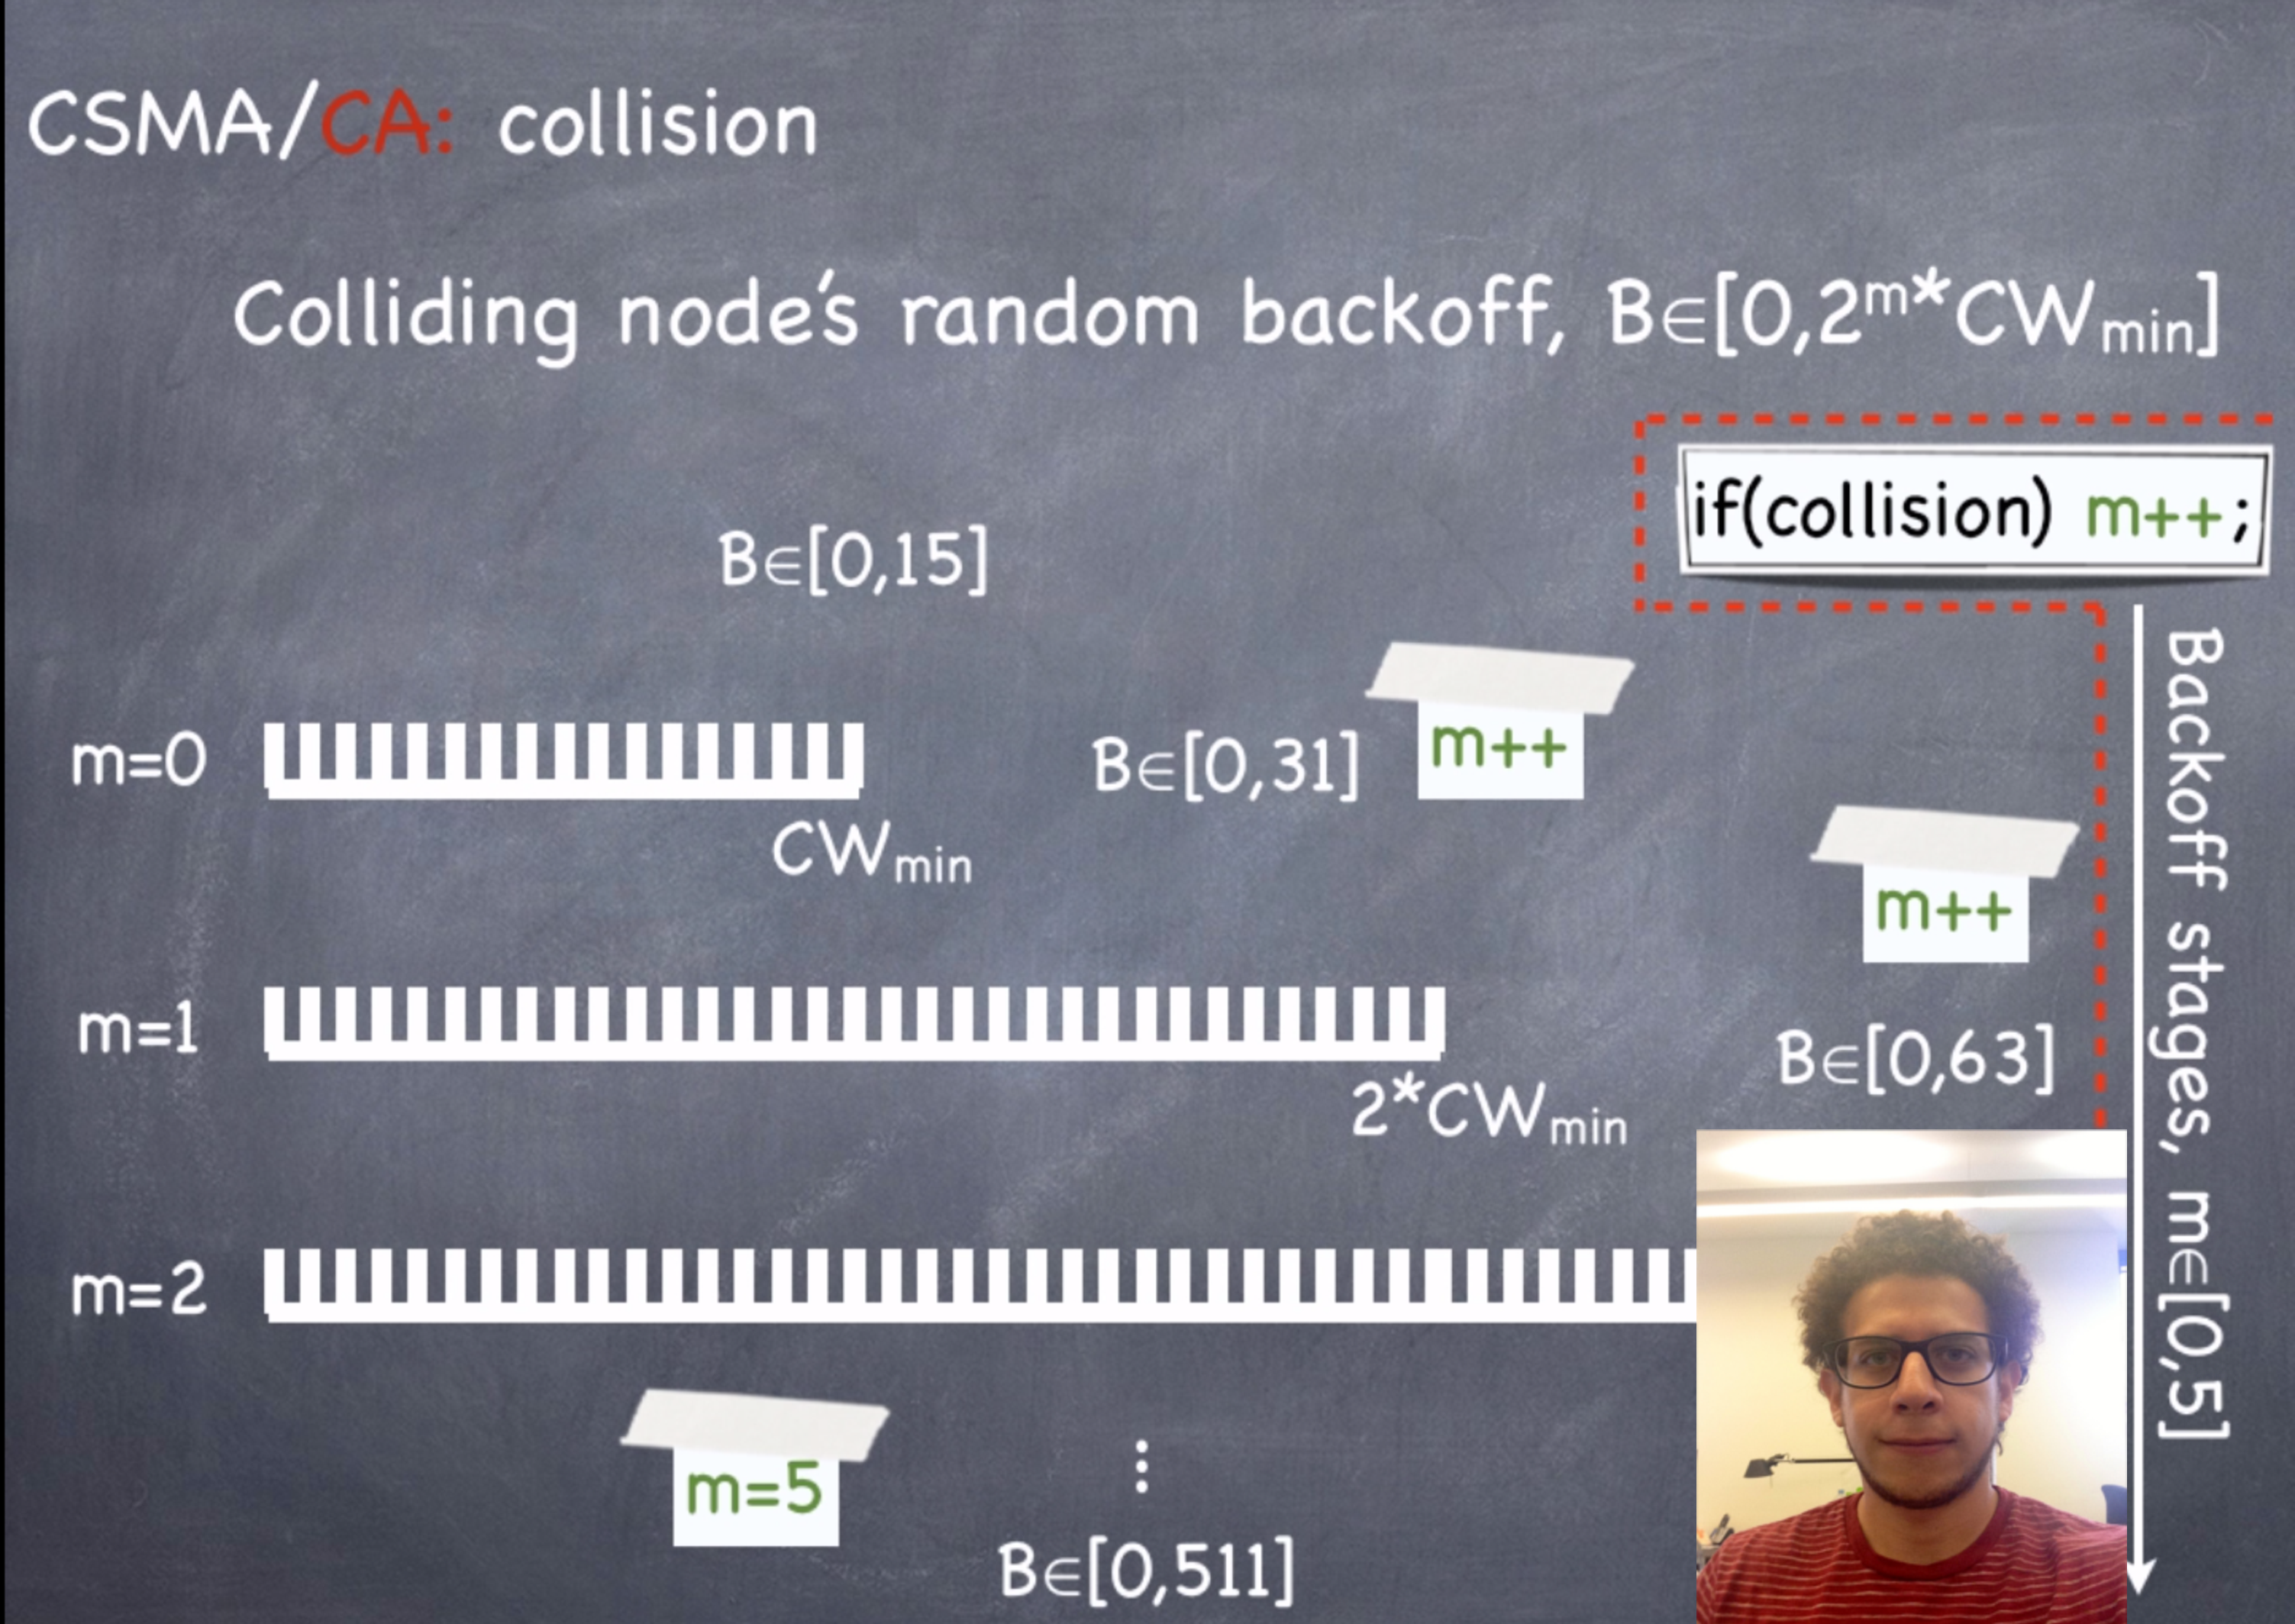
\includegraphics[width=\linewidth]{lesson}
\caption{Most video lessons will show the teacher's face over supporting slides.}
\label{fig:lesson}
\end{marginfigure}

%------------------------------------------------

\chapter{Results and Impact}

This course builds upon successful experiences. There is already an existing course that received very good feedback from the students. Also, there is a degree thesis by one of the students that was presented in Battlemesh, Aalborg University, and caught the attention of the P2P Foundation. Furthermore, the idea of bottom-up smart cities implemented by Smart Citizen was applauded in Kickstarter and received over \$60,000 in crowdfunding. 

The hardware used in the course is the Digi XBee, that was also used in the best-selling book by Rober Faludi ``Building Wireless Sensor Networks''; and the Arduino. More than one million Arduino have been sold, confirming the success of their open business model.

The main goal of this course is to strengthen the community by teaching very basic skills to a large audience. After completing the course, the participants will be able to continue on their own with more advanced projects. 

It is a basic digital education for everyone. People with no or little background in technology will make their first steps into programming, electronics, and sensing projects.

Students successfully completing this course will posses the basic tools to contribute to the creation of bottom-up smart cities.

% This course builds upon successful experiences. There is already an existing course that received very good feedback from the students. There is also a degree thesis by one of the students that was presented in Battlemesh, Aalborg University, and attracted the attention of the P2P Foundation.
% 
% The idea of bottom-up smart cities implemented by Smart Citizen was applauded in kick starter and received over \$60,000 in crowdfunding. The hardware used in the course is the XBee that was also used in the best-selling book by Rober Faludi “Building Wireless Sensor Networks”. More than one million Arduino have been sold confirming the success of their open business model.
% 
% The main goal of this course is to strengthen the community by teaching very basic skills to a large audience. After completing the course, the participants will be able to continue on their own with more advanced projects. It is a basic digital education for everyone. People with no or little background in technology will be do the first steps in programming, electronics, and sensing projects.
% 
% People that have taken the course will be able to contribute to the creation of bottom-up smart cities.



%------------------------------------------------

\chapter{Teaching Plan}

 Concepts and competences acquired in the course:
\begin{itemize}
\item Bottom-up, peer-to-peer and community-oriented collaboration models
\item Sensors, actuators, sensor networks, open data, smart cities
\item Very basic electronics
\item Very basic microprocessor programming
\item Configuration of Digi XBee
\item ZigBee communication
\end{itemize}

Weekly organization:
\begin{enumerate}
\item Presentation of the participants, presentation of the course, motivation to take the course, dream about a personal project.
\item Introduction to Arduino. Arduino IDE. Input/output. \\\underline{Lab assignment}: Blinking LED project.
\item Introduction to XBee. Basic configuration of AT mode. \\\underline{Lab assignment}: ZigBee chat project.
\item Basic interaction. Make a measurement and react. \\\underline{Lab assignment}: Wireless Sunset Sensor project.
\item Open data. The importance of sharing the data. Open data platforms. \\\underline{Lab assignment}: Taking measures with a sensor and uploading them to the Internet.
\end{enumerate}

Motivating videos:
\begin{itemize}
\item Do-it-ourselves, Bottom-up, Sensors, Smart Cities:
Laia Albo, Michel Bauwens, Tiberius Brastaviceanu, Tomas Diez

\item Arduino (Blinking LED):
Massimo, (Jaume)

\item XBee (Chat):
Robert Faludi (Luis)

\item Interaction design (Sunset Sensor):
Alex Posada (Luis)

\item Open Data, Open Data platforms (Internet thermometer):
Albert Domingo, Manuel Palacin, (Alejandro Andreu)
\end{itemize}


%------------------------------------------------

\chapter{Team}

\begin{itemize}
\item Lead teacher: Luis Sanabria-Russo (Universitat Pompeu Fabra)
\begin{marginfigure}
\includegraphics[width=0.5\linewidth]{luis}
\caption{Luis Sanabria-Russo}
\label{fig:luis}
\end{marginfigure}
\item Other members of the team:
\begin{itemize}
\item Laia Albo (Universitat Pompeu Fabra)
\item Alejandro Andreu (Universitat Pompeu Fabra)
\item Massimo Banzi (Arduino)
\item Jaume Barcelo (Universitat Pompeu Fabra): He is a lecturer at Universitat Pompeu Fabra where he takes part in the Wireless Sensor Network course. He has also taught at Universidad Carlos III de Madrid were he took part in the opencourseware experience that published the class materials online. Together with Luis Sanabria, he has prepared the basic laboratory guide for the WSN course that has been shared with the community in GitHub. Jaume has taught more than 20 courses at the graduate and undergraduate level at two universities.
\begin{marginfigure}
\includegraphics[width=0.5\linewidth]{jaume}
\caption{Jaume Barcelo}
\label{fig:jaume}
\end{marginfigure}

\item Michel Bauwens (P2P Foudation)
\item Tiberius Brastaviceanu (Sensorica)
\item Tomas Diez (FabLab Barcelona)
\item Albert Domingo (Universitat Pompeu Fabra)
\item Robert Faludi (Digi International)
\item Manuel Palacin (Universitat Pompeu Fabra)
\item Alex Posada (Media Interaction Design Lab)
\end{itemize}
\end{itemize}



\backmatter

%----------------------------------------------------------------------------------------
%	BIBLIOGRAPHY
%----------------------------------------------------------------------------------------

\bibliography{bibliography} % Use the bibliography.bib file for the bibliography
\bibliographystyle{plainnat} % Use the plainnat style of referencing

%----------------------------------------------------------------------------------------

\printindex % Print the index at the very end of the document

\end{document}
